% $Id: patches.tex 8166 2020-09-17 19:18:02Z mskala $

%
% MSK 014 patch ideas
% Copyright (C) 2022  Matthew Skala
%
% This program is free software: you can redistribute it and/or modify
% it under the terms of the GNU General Public License as published by
% the Free Software Foundation, version 3.
%
% This program is distributed in the hope that it will be useful,
% but WITHOUT ANY WARRANTY; without even the implied warranty of
% MERCHANTABILITY or FITNESS FOR A PARTICULAR PURPOSE.  See the
% GNU General Public License for more details.
%
% You should have received a copy of the GNU General Public License
% along with this program.  If not, see <http://www.gnu.org/licenses/>.
%
% Matthew Skala
% https://northcoastsynthesis.com/
% mskala@northcoastsynthesis.com
%

\chapter{Patch ideas}

Here's a straightforward subtractive patch controlled by the left pitch CV
and gate.  Pitch CV is split by a multiple to control the Middle Path
oscillator (both sides, through normalling in that module) and the Coiler
VCF.  Gate CV is also split to control two ADSR envelopes, for the VCF
(second CV input) and the VCA.  This patch would work well with a MIDI
keyboard or a mouse plugged into the Gracious Host.  Using MIDI channel~2,
the combination of channels~8 and~9, or the two buttons of a mouse, this
patch could be expanded to control modular voices, with the left and right
sides more or less independent.

\nopagebreak\noindent
{\hspace*{\fill}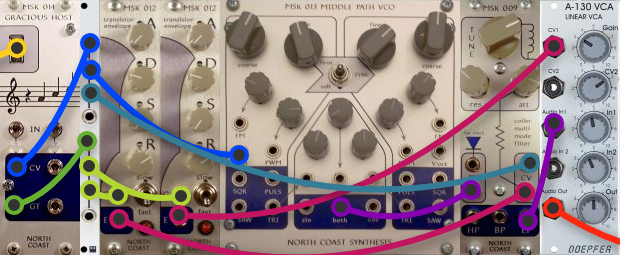
\includegraphics[scale=0.35]{patch1.png}\hspace*{\fill}\par} 

The next patch shows the ``non-USB'' behaviour of the Gracious Host:  with
nothing plugged into the USB port, it acts as a primitive oscillator and
envelope, taking pitch and gate CV as standard Eurorack control voltages and
producing a fixed-parameter ADSR envelope (upper right output jack) and
square wave oscillator output (lower left).  Here the Leapfrog VCF, with its
built-in VCA, is providing the rest of the patch (filtering and
articulation).  The quantized pitch CV output from the Gracious Host is
shown being used as the V/oct input for the filter to save the need for a
multiple, but it would also make sense to patch the original (unquantized)
pitch CV to the filter instead.

\pagebreak

This patch as shown will have a
significant DC offset on its output; any AC-coupled module, such as the AC
output of the MSK~011 Transistor Mixer, could remove that.

\nopagebreak\noindent
{\hspace*{\fill}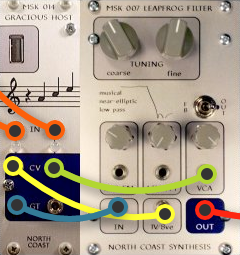
\includegraphics[scale=0.4]{patch2.png}\hspace*{\fill}\par} 

Here is a minimal patch intended to be controlled by a MIDI or typing
keyboard on MIDI channel~1, using the Gracious Host's built-in oscillator
feature.  The pitch CV controls the filter, the gate CV activates an ADSR
envelope, and the velocity CV goes to the filter's second CV input for
additional expressive control.  Another option might be to patch it to the
VCA to vary the volume.

\nopagebreak\noindent
{\hspace*{\fill}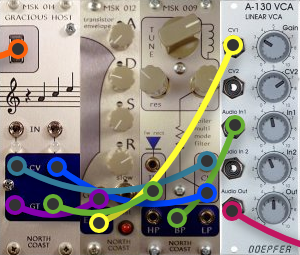
\includegraphics[scale=0.4]{patch3.png}\hspace*{\fill}\par} 

\pagebreak

This patch (really a partial patch) shows how the Gracious Host might be put
between a sequencer and an oscillator for MIDI-controlled quantization. 
Play several notes on MIDI channel~3 or~4 and the notes from the sequencer
will be shifted to the nearest MIDI notes; so a single sequence can play in
multiple keys or scales under keyboard control.  The left pitch CV is shown
dotted because this cable does not actually need to be patched; the Gracious
Host can send, and the Middle Path can receive, control voltages over the
Eurorack CV/gate bus.

\nopagebreak\noindent
{\hspace*{\fill}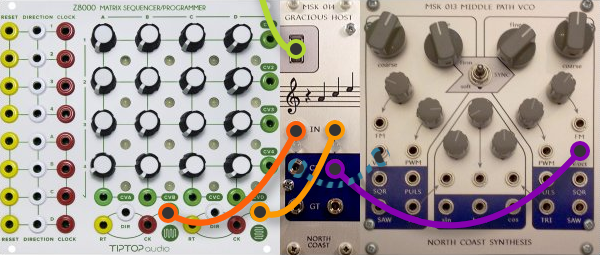
\includegraphics[scale=0.35]{patch4.png}\hspace*{\fill}\par} 

A USB mouse can be a general-purpose CV controller, not only used to play
notes.  In this patch it controls two volume levels with vertical and
horizontal movement, for mixing and cross-fading between two sampler
modules.  The gate outputs, shown unpatched, could be connected in a more
complicated patch to switch between samples.

\nopagebreak\noindent
{\hspace*{\fill}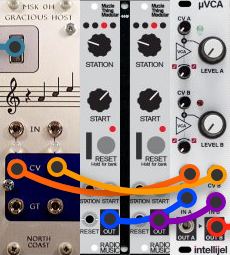
\includegraphics[scale=0.4]{patch5.png}\hspace*{\fill}\par} 
